\chapter[Referencial Teórico]{Referencial Teórico}

Esta sessão trará todo referêncial teórico necessário para desenvolver o projeto
de medição de débito técnico, contemplando tópicos explicativos sobre Débito Técnico,
Contratação e Medição e Análise.

\section{Débito Técnico}
Débito técnico é uma metáfora proposta por \cite{cunningham} onde uma dívida é
criada quando a qualidade do código é deixada de lado para acelerar o processo
de desenvolvimento, até o momento que esta dívida é quitada. O preço do pagamento
da dívida, geralmente feita através de refatoração, aumenta gradualmente com
a evolução do projeto.

\cite{oliveira} afirma que é possível identificar vários atributos em um Débito
Técnico, sendo eles:

\begin{itemize}
  \item \textit{Reason}, motivo pelo qual o débito foi adquirido;
  \item \textit{Benefits}, o lucro ou ponto positivo que a escolha de optar pelo débito traz;
  \item \textit{Result}, o que esse débito realmente possibilitou para a organização;
  \item \textit{Principal}, representa o preço que o pagamento do débito possui no momento;
  \item \textit{Interest}, preço de pagamento do débito depois de um dado tempo;
  \item \textit{Returns}, quanto a organização lucrou com a decisão de ter optado pelo Débito Técnico.
\end{itemize}


De acordo com \cite{mapping}, há um debate sobre a importância de gerenciar o
Débito Técnico, dada a importância deste para a equipe de negócios,
complementando que nem sempre este é ruim e que pode-se obter benefícios
que são maiores do que a perda monetária causada pelo juros.

\cite{mapping} identificam que o Débito Técnico tem atividades que podem ser classificadas.
Ela lista oito tipos de Débito Técnico, sendo eles:

\begin{itemize}
  \item Identificação;
  \item Medição;
  \item Priorização;
  \item Prevenção;
  \item Monitoramento;
  \item Pagamento;
  \item Representação/Documentação;
  \item Comunicação;
\end{itemize}

Quando se trata de Débito Técnico, existem modelos de identificação e medição de
código. O autor \cite{eisenberg} executa uma análise estática e utiliza o
resultado para estimar o quanto custará para sanar todo ou parte do Débito
Técnico existente em um projeto.



\subsection{Método SQALE para avaliação de Débito Técnico}
\cite{letouzey} propõe a utilização do método SQALE (\textit{Software Quality Assessment
based on Lifecycle Expectations}) para análise do débito técnico. O método de
Letouzey propõe um Modelo de Qualidade (\textit{SQALE Quality Model}) e um Modelo de
Análise (\textit{SQALE Analysis Model}) para verificação das violações de código.

O Modelo de Qualidade do SQALE constitui de uma matriz hierárquica de 3 níveis:
Características, Sub-Caracteristicas e Requisitos. Numa estratégia de análise de
débito técnico, pode ser definido que qualquer não-conformidade do código com os
requisitos caracteriza débito técnico. Por isso, os Requisitos devem ser atômicos,
não-ambíguos, não-redundantes, justificáveis, aceitáveis, implementáveis e
verificáveis.

Assim, basta utilizar uma ferramenta que consiga avaliar o código com relação
aos requisitos estabelecidos e será possível identificar o débito técnico na
aplicação.

O Modelo de Análise faz uso de um índice de remediação para avaliar os
impactos das violações identificadas. Esse índice de remediação faz uma relação
entre os Requisitos do Modelo de Qualidade, com uma remediação associada a
cada violação desses requisitos. Por fim, é estipulada, também, uma função de
remediação, que associa um tempo para aplicar aquela remediação.

\subsection{Identificação de Débito Técnico}
Para mensurar o débito técnico existente em uma aplicação é necessário que haja
meios de identificá-lo. Existem vários métodos de identificação de débito técnico,
sendo um deles o proposto por \cite{siebra}, afirmando que os resultados obtidos a
partir da medição de um conjunto de dez métricas podem identificar o quanto de
débito técnico uma aplicação possui. Essas métricas podem ser:

\begin{enumerate}
  \item Acoplamentos Aferentes;
  \item Acoplamentos Eferentes;
  \item Árvore de Profundidade de Herança;
  \item Falta de Coesão em Métodos;
  \item Número de filhos;
  \item Complexidade Cliclomática;
  \item Duplicação de Código;
  \item Documentação do Código;
  \item Métodos por classe;
  \item Acoplamento entre métodos.
\end{enumerate}

\subsection{Medição de Débito Técnico}
\cite{principal} propõem uma fórmula para identificação do principal de um
débito técnico, com parâmetros ajustáveis de acordo com os interesses da
organização. A formula é:

\begin{figure}[h]
  \centering
  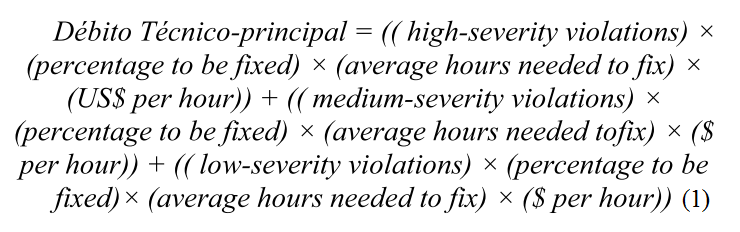
\includegraphics[width=250px, scale=1]{figuras/formulaprincipal}
  \caption{Cálculo do TD principal}
\end{figure}
Onde:

Débito Técnico-Principal: É o valor atual de Débito Técnico no \textit{software};

\textit{X-Severity-Violations}: O somatório total de números de ocorrências de violações
de uma severidade X;

\textit{Percentage to be fixed}: O percentual que a organização estipulou que irá corrigir
de violações daquele nível de severidade;

\textit{Average hours needed to fix}: Média do tempo necessário para corrigir uma violação
daquele nível de severidade;

\$ \textit{per hour}: Custo/hora de quem irá corrigir as violações.

Segundo os autores, com a fórmula, é possível obter o custo para corrigir o débito
técnico de um \textit{software}, de acordo com os parâmetros da organização.

Vale ressaltar que as definições dos níveis de severidade das violações (e seus respectivos pesos) são feitas pela organização que está a utilizar o método proposto.
Na figura apresentada acima, os termos \textit{high-severity violations}, \textit{medium-severity violations} e \textit{low-severity violations} são apenas exemplos representativos e poderiam indicar, por exemplo, os pesos 3, 2 e 1, respectivamente.

\section{Contratação na Administração Pública Federal Brasileira}

No Decreto-Lei nº 200, \cite{decreto200} institui princípios fundamentais para a
Administração Pública, sendo um deles a contratação de terceiros, que deve ser
executada sempre que houver possibilidade.

O decreto nº 2.271, por \cite{decreto2271}, aconselha que todos os produtos e seviços
que não tenham ligação direta para a utilização na organização, incluindo serviços
de informática, sejam terceirizados; a fim de destituir a responsabilidade do
órgão para com o desenvolvimento de vários serviços, privando-o unicamente com
a administração destes.

\section{Medição e Análise}
Em geral, medição é o processo no qual números ou símbolos são atribuídos a
atributos ou entidades do mundo real de forma a descrevê-los de acordo com regras
bem definidas \cite{fentonpfleeger}. O resultado númerico é chamado 'medição'.
Isto pode ser aplicado ao desenvolvimento de \textit{software} e ao produto de \textit{software}.

Medição de \textit{software} é um processo contínuo de definição, coleta e análise de
dados em cima do desenvolvimento de \textit{software} e seus produtos com o objetivo de
entender e controlar o processo \cite{egon}.


Em seu livro \textit{Software Metrics - A Rigorous and Practical Approach}, Fenton define
medição como o processo de atribuição de números ou símbolos que são atribuídos
a atributos de entidades do mundo real, para descrever elas de acordo com regras
definidas. Ele ainda nos diz que uma entidade pode ser tanto um objeto, quanto
um evento do mundo real, e um atributo é uma característica ou propriedade dessa
entidade que nos interessa.

Ele ainda define que existem dois tipos de quantificação: Medição e Calculação.
A medição é direta, como medir o peso de alguém. Já a calculação é indireta, onde
são realizadas medições e a combinação delas refletem o atributo que estamos
tentando entender.

A medição se faz necessária em um projeto de \textit{software} pois ela nos auxilia a
entender o que está acontecendo, o que nos permite ter um controle maior sobre o
projeto e melhorar o mesmo.

\subsection{Objetivos da medição de \textit{software}}
Medição é uma ferramenta poderosa para entender os efeitos das ações que são
tomadas para melhorar o processo de desenvolvimento de \textit{software}
\cite{egon}.

Dados de medição de \textit{software} são interpretados para prover informações que podem
ser aplicadas para três diferentes propósitos. Em primeiro lugar, os dados
fornecem visibilidade do processo de desenvolvimento atual e as características
dos produtos de \textit{software}. Essa visibilidade é requerida para reduzir a complexidade
e aumentar o entendimento do processo e dos produtos. Entedimento significa
determinar as diferentes variáveis que existem durante a execução de um processo.
Uma vez que um entedimento básico é estabelecido, os dados coletados e analisados
podem ser usados para controlar o processo e os produtos. Isso significa que as
relações entre os variáveis de processos têm de ser determinadas. Uma vez que
 essas relações são conhecidas, elas podem ser usadas parar controlar o processo.
 Além disso, baseados em análise, os dados de medição coletados podem ser usados
 para avaliar o processo e, então, agir como indicadores das áreas problemáticas
 do processo de desenvolvimento, do qual ações de melhoria podem ser tomadas
 \cite{pfleeger}.

\subsection{Conceitos de medição de \textit{software} orientada a meta}
Medição de \textit{software} só deve ser realizada diante de propósitos bem definidos.
A medição de \textit{software} orientada a meta é especialmente usada para programas de
 melhoria. O método aplicado nesse trabalho é o método GQM (\textit{Goal, Question, Metric})
 concebido por \cite{basiliRombach}.

 O método GQM contém quatro fases:
\begin{enumerate}
  \item   \textbf{Fase de planejamento}, onde a escolha do projeto para a aplicação de
  medição é selecionado, definido, caracterizado e planejado;
  \item  \textbf{Fase de definição}, onde o programa de medição é definido (metas, questões,
  métricas e hipóteses são definidas) e documentado;
  \item  \textbf{Fase de coleta de dados}, onde a a coleta de dados realmente acontece;
  \item  \textbf{Fase de interpretação}, onde os dados coletados são processados de
  acordo com as métricas definidas nos resultados de medição, que provêm
  respostas para as questões definidas.
\end{enumerate}

A fase de planejamento é executada para obter os requisitos básicos para a
construção de um bom GQM, incluindo treinamento, envolvimento de gerência e
planejamento de projeto. Durante a fase de definição, todos os entregáveis do
GQM são desenvolvidos, baseados, principalmente, em entrevistas estruturadas.
Na fase de definição, também são identificados os objetivos, todas as questões,
métricas relacionadas e hipóteses das medições. Durante a fase de coleta de
dados, as formas de coletar dados são definidas e preenchidas em um banco de
dados de medição. Então, o trabalho, de
fato, pode começar: usando os dados de medição. Durante a fase de interpretação,
as medições são usadas para responder as questões propostas e essas respostas são,
novamente, para verificar se as metas propostas foram atingidas \cite{egon}.


\subsection{Escalas}
\cite{fenton} nos diz que nem todos os tipos de medição são iguais em seu mapeamento
entre o mundo real e o mundo abstrato. Assim, existe o conceito de escala de
medição que visa abordar essa diferença entre as medições. \cite{fenton} traz principalmente
5 grandes classificações, quer seriam nominal, ordinal, intervalar, racional e
absoluta.

A escala nominal atribui um nome ou um rótulo ao atributo, não existindo noção
de ordem ou magnitude entre elas.

A escala ordinal se assemelha a anterior mas nesta existe a noção de ordem. Caso
seja utilizado números eles servem apenas para propósitos de classificação, não
sendo possível realizar operações matemáticas entre eles.

A escala intervalar preserva a noção de ordem dos resultados e ainda traz noções
de intervalo que separam seus pontos. É possível realizar adição e subtração, mas
não multiplicação e divisão.

A escala racional possui a noção de ordem e intervalos e ainda incorpora a noção
de razão. Também está presente o zero absoluto, que significa a ausência do atributo.
Todas as operações aritméticas podem ser utilizadas para essa escala.

A escala absoluta é um tipo especial da escala racional, onde são admitidos apenas
multiplicadores unitários, gerando assim números absolutos. Deve ser obtido
através da contagem.


\subsection{Conceito de medição: o paradigma GQM}
O GQM representa uma abordagem sistemática para confeccionar e integrar metas a
modelos de processos de \textit{software} e produtos, baseada em necessidades específicas
do projeto e da organização \cite{basiliRombach}. O resultado da aplicação do
método GQM é a especificação de um programa de medição que mira um conjunto de
pontos e um conjunto de regras para a interpretação de dados de medição.

O princípio por trás do método GQM é que a medição deveria ser orientada a metas.
Assim, para melhorar um processo, organizações devem definir suas metas de medição
baseadas em objetivos corporativos e transformá-las em atividades que podem ser
 medidas durante a execução do projeto \cite{egon}.

O GQM define uma certa meta, sintetiza essa meta em questões, e define métricas
que devem prover informações para responder essas questões. Ao responder essas
questões, os dados medidos definem as metas operacionalmente, e podem, então,
ser analisados se as metas foram cumpridas. Assim, o GQM define métricas por uma
perspectiva \textit{top-down} e analisa e interpreta os dados de medição de uma maneira
\textit{bottom-up}.

O modelo GQM começa de uma maneira \textit{top-down} com a definição de uma meta de medição
explícita. Essa meta é sintetizada em várias questões que quebram o problema em
componentes maiores. Cada questão é, então, refinada em métricas que deviam prover
informações para responder aquelas várias questões. A medição de dados, por outro
lado, é interpretada de maneira \textit{bottom-up}. Como as métricas foram definidas com
uma meta explícita em mente, a informação provida pelas métricas devem ser
interpretadas e analisadas em respeito a essa meta, para concluir se ela foi
ou não cumprida \cite{egon}.
